%!TEX root = ../thesis.tex
%Adding the above line, with the name of your base .tex file (in this case "thesis.tex") will allow you to compile the whole thesis even when working inside one of the chapter tex files
%: ----------------------- introduction file header -----------------------
\chapter{Conclusions and Future Work}
\label{chap:8}

The goal of the thesis was to broaden and deepen our understanding of the outflow environments of red giants and red supergiants. To achieve this goal, we observed these stars with the most sensitive radio interferometers available, allowing their atmospheres to be probed with excellent detail. The first part of the thesis described the results of our multi-wavelength high spatial resolution campaign to enhance our understanding of Betelgeuse's complex outflow environment. The second part of the thesis focused on the analysis of multi-wavelength centimeter continuum emission from Arcturus and Aldebaran, which provided a snapshot of the different stellar atmospheric layers. In this chapter, the primary findings and conclusions of these two studies are presented along with possible directions for future work.

\pagebreak

\section{Principle Results}\label{sec:8.1}
The main findings of the thesis are discussed in the following two sections.
\subsection{Multi-wavelength Study of Betelgeuse's Extended Atmosphere}\label{sec:8.1.1}

\begin{itemize}

\item The two distinct velocity components seen by \cite{bernat_1979} in CO absorption against the stellar spectrum at 4.6 $\mu$m were both separately detected and spatially resolved at 230\,GHz for the first time. The extended CARMA C configuration resolved out almost all of the S2 emission leaving us with an approximate line profile for the S1 flow. From this profile a blueshifted outflow velocity of $-9.0\>{\rm km\>s}^{-1}$ and a slightly greater redshifted outflow velocity of $+10.6\>{\rm km\>s}^{-1}$ was inferred; in good agreement with \citeauthor{bernat_1979}'s (\citeyear{bernat_1979}) line of sight expansion velocity value of $-9\>{\rm km\>s}^{-1}$.  

\item The line profiles obtained with the D and E configurations were found to be wider than the C configuration line profile, with the notable appearance of an extreme blue wing feature which was associated with the S2 flow. The high spectral resolution multi-configuration spectrum was used to determine S2 outflow velocities of $-15.4\>{\rm km\>s}^{-1}$ and $+13.2\>{\rm km\>s}^{-1}$, which are in good agreement with \citeauthor{bernat_1979}'s (\citeyear{bernat_1979})  value of $16\>{\rm km\>s}^{-1}$.  

\item In the blueshifted channels of the  multi-configuration image cube the emission is compact at high absolute velocities and becomes more extended at lower absolute velocities, indicating that the S2 flow has a shell like structure. This is less clear in the redshifted channels, indicating an asymmetric shell. These multi-configuration maps provide the first direct measurements on the spatial extent of the S2 flow, which we derive to have a radius of 17$\arcsec$; a value that is higher than most previous single dish estimates. 

\item A well defined outer edge for the S1 flow is not obvious. The emission at low absolute velocities is resolved out in the S1 line profile and because the resolving out scale of the C configuration is $\sim 6\arcsec$, this tells us that the spatial extent of the emission must be at least $\sim 3\arcsec$. From the intensity distribution of the S1 emission, we infer that the extent of the S1 emission is between $4-6\arcsec$.

\item Both flows were found to be inhomogeneous down to the resolution limit, with a notable clump of emission $\sim 5\arcsec$ S-W of the star, at low absolute velocities in the stellar rest frame. However, when azimuthally averaged, the intensity falloff of both flows were found to be consistent with an optically thin, spherically symmetric constant velocity outflow, similar to that found for K\,I at larger scales.

\item Previous single dish observations of the CO line with small HPBWs do not show the classical resolved signature of high emission at large absolute velocities and low emission at low absolute velocities for two main reasons. Firstly, the S1 flow is still unresolved in these single dish observations and thus contributes emission at the lower absolute velocities. In addition, the multi-configuration CARMA maps show that the S2 emission is brighter in the higher absolute velocity maps than at lower absolute velocities and so when the emission from the fainter rings is neglected (i.e. when observed with a small HPBW), the overall line profile does not change significantly.

\item The various CO rotational line profiles get narrower with increasing excitation energies, indicating that the higher excitation lines are formed mainly in the S1 flow. Therefore the high frequency bands of ALMA will preferentially trace the S1 flow. 

\item Assuming a mean outflow velocity of $14.3\>{\rm km\>s}^{-1}$ and $9.8\>{\rm km\>s}^{-1}$ for the S2 and S1 flows, respectively, then their ages are $\sim 1100$\,yr and $\sim 400 \rightarrow 600$\,yr. The S1 flow may be an extension of the current wind phase seen at UV and centimeter wavelengths, but higher spatial resolution data is needed to confirm this (see Section \ref{sec:8.2.1}).

\item The thermal continuum emission of Betelgeuse's inner atmosphere has been imaged at 6\,cm with e-MERLIN, revealing two unresolved hotspots separated by 90\,mas, with brightness temperatures $5400\pm 600$ and $3800\pm 500$\,K. The astrometric solutions of \cite{harper_2001} place the optical photospheric position almost directly at the position of the weaker feature, meaning that the hotter feature is $\sim 2\,R_{\star}$ above the optical photosphere. Existing 1-D atmospheric models are capable of almost reproducing the low resolution e-MERLIN image, but are inadequate at the highest e-MERLIN resolution. 1-D atmospheric models are probably not a realistic representation of Betelgeuse's inner atmosphere.

\item High spatial resolution multi-wavelength archival VLA+Pi Town data, taken 10\,yr prior to the e-MERLIN data set, were examined to look for signatures of the e-MERLIN hotspots. No evidence was found for the presence of the two hotspots at either 1.3 or 0.7\,cm where the resolution was comparable or better than that of e-MERLIN's. We conclude that the hotspots are either optically thin at these high frequencies or their dynamics are time dependent on scales of just a few years.

\item Multi-epoch, multi-wavelength radio continuum observations between 1996 and 2004 reveal total flux density variations between $20\rightarrow 35\%$ at wavelengths between 0.7 and 6\,cm. The 0.7\,cm radio maps show a highly asymmetric source at all epochs, with dramatic changes in the radio emitting topology over a time period of only one to two years. These frequent changes in the radio emitting topology may be the cause of the flux density variations at 0.7\,cm.
  
\end{itemize}


\subsection{Multi-wavelength Radio Continuum Emission Studies of Dust-free Red Giants}\label{sec:8.1.2}

\begin{itemize}
	\item The thesis has presented the most comprehensive set of multi-wavelength radio continuum observations of two luminosity class III red giants to date. A snapshot of the different stellar atmospheric layers of Arcturus and Aldebaran was obtained, independent of any long-term variability. The first detections were made at several wavelengths for each star, including a detection at 10\,cm (3.0 GHz: S band) for both stars and a 20\,cm (1.5 GHz: L band) detection for Arcturus, making these the first isolated luminosity class III red giants to be detected at such long wavelengths.
  
	\item The long-wavelength data sample the outer layers of Arcturus' atmosphere where its wind velocity is approaching its terminal value and the ionization balance is becoming frozen-in. For Aldebaran however, the long-wavelength data is still sampling its inner atmosphere where the wind is still accelerating, probably due to its lower mass loss rate. 

	\item Little evidence for radio flux variability was found when our measurements were compared with previous observations. However, previous observations have provided only a small number of modest S/N measurements and so it is difficult to make a conclusive statement regarding the radio variability of these sources. Interestingly, prior to this study Aldebaran had been observed at 6\,cm but was not detected. However, we detected the star at 6\,cm with a flux density over two times greater than the previous $3\sigma$ upper limit, which could mean that its wind may have a time dependent nature.
	  
	\item Our radio flux density measurements were compared with the predictions of published semi-empirical models based on UV data. The chromospheric and transition region semi-empirical model of \cite{mcmurry_1999} with an optically thin wind overlain does well in reproducing our radio fluxes but we find that the chromospheric and wind semi-empirical model of \cite{drake_1985} does not agree well with our data.
  
	\item Arcturus was found to have a spectral index of $\alpha = 1.05 \pm 0.05$ while Aldebaran's value was found to be higher at $\alpha = 1.58 \pm 0.25$. Both of these values are well above that expected for an isothermal wind with a constant velocity and ionization fraction.

	\item The long wavelength radio measurements of Arcturus were found to be emanating from a region of the atmosphere where its wind is close to the terminal velocity. This allowed evidence to be found for a rapidly cooling wind with a temperature, $T(r) \propto r^{−1.65}$.
	
	\item A new wind model was developed for Arcturus which was based on the analytical advection model of \cite{glassgold_1986}. It incorporates a rapidly cooling wind profile and was based on the new VLA long wavelength flux measurements. This provided a new \textit{hybrid} atmospheric model for Arcturus, which consists of the original inner atmosphere developed by \cite{drake_1985}, out to a radius of $2.3\,R_{\star}$ and the new wind model farther out.

	\item The new hybrid atmospheric model for Arcturus was used to investigate the various heating and cooling processes that control the thermal structure of its mass outflow region between $1.2\rightarrow  10\,R_{\star}$. Lyman $\alpha$ line cooling was found to be the main cooling mechanism within $2.8\,R_{\star}$ while adiabatic expansion cooling was the most efficient cooling mechanism farther out. Magnetic wave heating is found to be the likely main heating mechanism throughout the atmosphere. A considerable net cooling was calculated at all distances from the star. Within $\sim 3\,R_{\star}$, this net cooling far exceeds that predicted by the atmospheric model, implying that one or more additional energy inputs must be acting on the inner region of the outflow to maintain the thermal profile. Beyond $\sim 3\,R_{\star}$, the only significant cooling process is adiabatic expansion, which is insufficient to account for the super-adiabatically cooling wind.

\end{itemize}

\section{Future Work}\label{sec:8.2}
The research presented in this thesis highlights the important and exciting science which can be carried out with red giants and red supergiants at radio wavelengths, using the latest suite of radio interferometers. The main findings presented in this thesis have been based on observations carried out with the most sensitive millimeter and centimeter interferometers available at the time. The CARMA millimeter interferometer is currently being surpassed in sensitivity, spatial and spectral resolution, and frequency coverage by the Atacama Large Millimeter/submillimeter Array (ALMA). ALMA will open up a whole new part of the millimeter and submillimeter spectrum for study with  unparalleled detail, allowing the distribution of molecules and dust around M supergiants to be mapped with resolution of just a few milliarcseconds at the highest frequencies. Most of the centimeter observations discussed in this thesis were obtained with the VLA and e-MERLIN during their commissioning phase with only a fraction of the now available bandwidth. The large bandwidth now available with these instruments will  allow fast detections of historically weak or undetectable radio continuum luminosity class III red giants at both long and short wavelengths. Previous upper limits will be replaced by firm detections allowing a greater understanding of their outer atmospheric properties. In the following sections we describe some future projects which would complement and improve on the work presented in this thesis.

\subsection{Probing the S1 flow of Betelgeuse with ALMA}\label{sec:8.2.1}
Chapter \ref{chap:5} outlined how the inner S1 flow around Betelgeuse was successfully imaged with sub-arcsecond spatial resolution (i.e., $0.9\arcsec$), revealing an irregular CO distribution between $40\,R_{\star}$ ($0.9\arcsec$) and $270\,R_{\star}$ ($\sim 6\arcsec$). Recently, \cite{kervella_2011} recorded a series of thermal IR images using the VLT/VISIR ($\lambda = 8-20\,\mu$m) and found a ring-like structure at radius $0.5-1.0\arcsec$ (i.e., $\sim 30\,R_{\star}$), which the author associated with the dust condensation radius. Such a spatial scale was just beyond the resolution of our CARMA data set. To build a complete and consistent picture of the mass-loss in Betelgeuse were awarded 5.5 hours of observing time with ALMA in the current observing cycle (i.e., ALMA Early Science Cycle 1). The goal of this scheduled study is to unravel the dynamical and chemical structure of the inner ($\lesssim 3\arcsec$) CSE, via observations of molecular line emission with a resolution of $\sim 0.09\arcsec$, an order of magnitude greater than our CARMA study. Such observations will shed light on the spatial correlation between the dust and molecules in the CSE and may identify the region where molecules condense into dust grains.

\begin{figure}[!ht]
\centering 
        \includegraphics[trim=0pt 310pt 0pt 280pt,clip, width=15cm,height=7cm]{/home/eamon/thesis/thesis_template/8/dust_alma.ps}
\caption[Simulating ALMA dust observations]{\textit{Left:} Dust emission model based on the the VLT/VISIR image of \cite{kervella_2011} showing a ring like structure which may be the region of dust condensation around Betelgeuse. \textit{Right:} Simulated ALMA image of 6\,GHz of continuum emission after two hours on source reveals that some of the structure should be detectable. }
\label{fig:8.1}
\end{figure}

\begin{figure}[!ht]
\centering 
        \includegraphics[trim=0pt 310pt 0pt 280pt,clip, width=15cm,height=7.2cm]{/home/eamon/thesis/thesis_template/8/co_alma.ps}
\caption[Simulating ALMA CO(J=6-5) observations]{\textit{Left:} Channel map from the CO($J=2-1$) image cube of \cite{ogorman_2012} using CARMA with a resolution of $0.9\arcsec$. \textit{Right:} CASA simulator tool image of the CARMA channel map scaled according to the Herschel CO($J=6-5$) emission line flux (see Chapter \ref{chap:5}) while assuming to have structure on the same scales as the dust. The scaling on the axes are different in both images.} 
\label{fig:8.2}
\end{figure}

The observations will be carried out in the $B_{\rm{max}} \sim 1\,$km configuration and the main target line will be the CO($J=6-5$) line at 691\,GHz. CO is a very stable molecule and does not take part in dust condensation allowing us to distinguish between different chemical and dynamics effects. Figure \ref{fig:8.1} displays a dust emission model based on the the VLT/VISIR image of \cite{kervella_2011} showing a ring like structure which may be the region of dust condensation around Betelgeuse. The CASA simulation tool was then used to create an image of the expected ALMA dust observations, assuming 6\,GHz of line-free continuum close to 690\,GHz. In just 2 hours of observing time we expect to be able to detect at least some of this structure. Figure \ref{fig:8.2} (left) shows a channel map from our final CARMA CO($J=2-1$) image cube. We scaled the intensity of this map according to the Herschel CO($J=6-5$) line flux and assumed that the CO has structure on the same scales as the dust. Figure \ref{fig:8.2} (right) shows the simulated distribution and brightness of the CO($J=6-5$) which indicates that we will be able to locate individual clump emission with a $0.09\arcsec$ beam. Even though the S1 flow is expected to extend out to $\sim 6\arcsec$, the CO($J=6-5$) will be more concentrated than the CO($J=2-1$) emission and so most of the  CO($J=6-5$) emission will be within the $9\arcsec$ ALMA primary beam. The flexibility of the ALMA correlator will also allow some other high-excitation lines to be simultaneously observed, such as SiO($v=0, J=16-15$) and SiO($v=1,J=16-15$) enabling the role of SiO in the formation of silicate dust grains to be studied. 

\subsection{Multi-epoch centimeter observations of Betelgeuse}\label{sec:8.2.2}
The recent e-MERLIN 5.2\,cm continuum image of Betelgeuse by \cite{richards_2013} has made the surprise discovery that the inner atmosphere contains two hotspots separated by 90\,mas (i.e., $4\,R_{\star}$). A number of outstanding issues remain in explaining the origin of these features. The first issue is that the exact position of the optical photosphere is uncertain. While \cite{richards_2013} assumed this position to be at the source peak of a lower resolution image, we have shown that the astrometric solution of \cite{harper_2008} places the optical photosphere almost directly at the position of the less bright hotspot, which would mean that the brightest feature is located $\sim 3\,R_{\star}$ above the optical photosphere. However, this astrometric solution was based in part on lower spatial resolution and S/N radio data and so does not contain the desired level of precision. Another issue is that the time scales over which these features vary, in both brightness and position, are completely unknown.  Along with the uncertainty in the photospheric position, the problem is that the velocity profile of the inner atmosphere is uncertain, due to traditional UV line diagnostics being contaminated by the large turbulent velocity.

Our VLA$-$Pie Town data have revealed significant flux variations at all observed wavelengths on time scales as short as 14 months (the observing interval), while \cite{drake_1992} found similar variations on time scales as short as 40 days. The source of these variations will probably be strongly associated with these hot spots, at C band at least, as \cite{richards_2013} have shown that these contain most of the total radio flux. \cite{ohnaka_2011} created a 1-D aperture synthesis image of Betelgeuse using the VLTI/AMBER and concluded that  ``\textit{the outer atmosphere extending to $\mathit{\sim 1.3 - 1.4\,R_{\star}}$ is asymmetric and its dynamics is dominated by vigorous, inhomogeneous large-scale motions, whose overall nature changes drastically within one year}''. Could it be possible that the hotspots seen at radio wavelengths also  change drastically within one year? Either way, they are likely linked to the wind-driving mechanism.

\begin{table}[hb]
\begin{center}
\caption[Relevant capabilities of the VLA and e-MERLIN]{Relevant capabilities of the VLA and e-MERLIN for future multi-epoch observations of Betelgeuse}
\begin{tabular}{ccccc}
\hline
\hline
\rule{0pt}{2.5ex}  & e-MERLIN  & e-MERLIN & VLA  & VLA \\
\rule{0pt}{2.5ex}  & (C band) & (K band) & (C band) & (K band)\\
\hline
\rule{-2.5pt}{2.5ex}	Resolution$^{1}$ (mas) &  40 & 12 & 330&90\\
					Frequency range (GHz) &  $4-8$ & $22-24$ & $4-8$&$18-26.6$\\
					Bandwidth (GHz) &  2& 2 & 4&8\\
					Sensitivity$^{2}$ ($\mu$ Jy/bm) & $\sim 2$ & $\sim 15$&$\sim 2$&$\sim 2$\\
					Maximum Scale ($\arcsec$) & $\sim 0.75$ & $\sim 0.16$&$\sim 8.9$&$\sim 2.4$\\
\hline
\end{tabular}
\label{tab:8.1}
\begin{minipage}{12.5cm}
\rule{-2.5pt}{2.5ex}{\footnotesize $^{1}$\,Using uniform weighting. $^{2}$\,Eight hour observing run.}
\end{minipage}
\end{center}
\end{table}

Spatial resolution is a key requirement to understand the dynamics and evolution of these hotspots and e-MERLIN is the most suited instrument for future radio studies. e-MERLIN is expected to operate at K band by 2014 and so a future study consisting of both C and K band observations would be preferable, as each frequency would probe different layers of the atmosphere, potentially detecting other unique hotspots. Table \ref{tab:8.1} summarizes the relevant capabilities of e-MERLIN for such a study. The additional K band observations would provide a maximum resolution of 12\,mas providing $\sim 10$ resolution elements across the radio disk\footnote{Based on the diameter of the fitted circular disks of our K band VLA+Pie Town data.}. Multi-epoch observations will be required to study the evolution of these features. Based on the conclusions of \cite{ohnaka_2011} along with the substantial flux variations we see in the radio, it would seem appropriate to carry out $3-4$ unique observations at both C and K band in one year. \cite{richards_2013}  C band observations were approximately 10\,hr in total duration and used a total bandwidth of 0.5\,GHz. Assuming the availability of the full 2\,GHz of bandwidth at both C and K band then, in order to reach similar levels of sensitivity, three unique epochs each consisting of C and K band observations would amount to 30 hours of requested time with e-MERLIN.

\begin{figure}[!ht]
\centering 
        \includegraphics[trim=0pt 170pt 0pt 150pt,clip, width=15cm,height=12.0cm]{/home/eamon/thesis/thesis_template/8/rhys_morris.ps}
\caption[MERLIN $+$ ``old'' VLA image of Betelgeuse]{Combined MERLIN and ``old'' VLA image of Betelgeuse at C band. The MERLIN data were taken between $3-5$ and $13-14$ November 1996, while the VLA data were obtained on the 21st October, one and two weeks prior to the MERLIN data. The maximum resolution is 57\,mas and the contour levels are at $(1,2,3,4,5)\times 90\,$mJy. Extended emission exits on scales of $\sim 400$\,mas while the inner emission is asymmetric in the same direction as the new e-MERLIN data, although the distribution of the intensity appears to be different. The recent upgrades to e-MERLIN and the VLA now provide $\sim 20$ and $\sim 40$ times more bandwidth, respectively, than that used in this image. Figure taken from \cite{morris_2001}.} 
\label{fig:8.3}
\end{figure}

Figure \ref{fig:8.3} shows a combined MERLIN and ``old'' VLA image of Betelgeuse at C band from 1996. Extended emission exits on scales of $\sim 400$\,mas while the inner emission is asymmetric in the same direction as the new e-MERLIN data, although the distribution of the intensity appears to be different. Extended emission was also detected in the e-MERLIN map in the form of a S-W arc at $\sim 250$\,mas from the star, as described in Chapter \ref{chap:6}. The shorter baselines of the VLA would be more sensitive to this extended emission than e-MERLIN and so, combining VLA data with e-MERLIN data would surely produce the most detailed radio map of Betelgeuse ever produced. Obtaining contemporaneous observing time with both the VLA and e-MERLIN at C and K band will be a challenge, especially considering that both instruments are now dynamically scheduled. A more realistic option would be to apply for one epoch of VLA time to coincide with one of the e-MERLIN observing blocks. Besides, the extended emission evolves on slower timescales, and so one epoch would be sufficient to create a detailed map of the extended emission.

\subsection{Semi-empirical models for Arcturus and Aldebaran}\label{sec:8.2.3}

\begin{figure}[!]
\centering 
        \includegraphics[trim=0pt 50pt 0pt 30pt,clip, width=16cm,height=18.5cm]{/home/eamon/thesis/thesis_template/8/advec_outline.ps}
\caption[Block diagram for a new semi-empirical model]{Block diagram summarizing the various stages involved in developing a new semi-empirical model for Arcturus and Aldebaran. The input model (starting guess) is mainly based on UV diagnostics. The radiative transfer equation and non-LTE atomic level populations (which include advection) are then simultaneously solved, and a radio spectrum is computed from the densities which is compared to the VLA data. The input model is adjusted until the computed radio spectrum agrees with our VLA observations.} 
\label{fig:8.4}
\end{figure}

The new hybrid atmospheric model for Arcturus outlined in Chapter \ref{chap:6} can reproduce our VLA flux density values at long wavelengths (i.e., $\lambda \gtrsim 2\,$cm) but does still not reproduce radio fluxes at shorter wavelengths. The next step of this project is to develop an entirely new atmospheric model independent of other existing models. Such a model would be based on our multi-wavelength VLA data because, unlike traditional UV diagnostics which are sensitive to localized hot plasma components, the multi-wavelength radio measurements probe many different layers and are more sensitive to the mean radial electron temperature.

We are currently developing the tools required to build these model atmospheres and our approach is outlined in Figure \ref{fig:8.4}. A grid of wind models, with different wind acceleration profiles, mass-loss rates, and temperature profiles will be created as a starting guess, whose values will be based on our best estimates from line emission profiles in the optical and UV. The starting densities are found assuming spherical symmetry and a constant mass-loss rate. Of these input parameters, the temperature profile will be the most uncertain as there is no detectable wind emission feature in either the optical or UV. Future spatially resolved e-MERLIN observations of our two targets would be of great value as they would constrain the thermal profile. This input model is then used as a starting guess to to simultaneously solve the radiative transfer equation and non-LTE atomic level populations (i.e., the rate equations) which include advection. An approximate solution for the ionization balance is then found by using escape probabilities for the optically thick lines in a six level hydrogen atom, and assuming the flow to be steady, which removes the time derivative in the rate equation. The ionization solution is non-linear and finding suitable models is a challenging computational project. Once a solution to the ionization balance has then been found, the corresponding radio spectrum is generated using the same techniques as described in Chapter \ref{chap:6}. This radio spectrum is then compared against the actual VLA data and if it matches then this is the new atmospheric model; otherwise the process is started again with a slightly different starting guess.

%The code uses finite differences and way I solved the problem requires solving a tri-diagonal matrix where each element is a 6x6 atomic model for hydrogen.

\subsection{Karl G. Jansky VLA Survey of Coronal Evolved Stars}\label{sec:8.2.4}
Optically thin radio emission from coronal giants and supergiants can constrain exisiting atmospheric models and even provide estimates of their mass loss rates. The main survey of such stars was carried out by \cite{drake_1986} at 6\,cm with the old VLA. Many of their sample were known x-ray sources whose observed spectra could be well fit by optically thin, thermal emission models with $T_e \sim 10^6-10^{7.5}$\,K \citep{ayres_1981}. At radio wavelengths, this thermal emission is completely dominated by free-free processes, while at x-ray wavelengths, it is the sum of many different thermal processes such as free-free, free-bound, and bound-bound. \cite{drake_1986} showed that the observed x-ray flux, $f_{x}$, in the soft x-ray band of the \textit{Einstein} Observatory is theoretically related to the 6\,cm optically thin coronal radio flux, $F_{\mathrm{cor}}$, by
\begin{equation}\label{eq:8.1}
1\times 10^6 \sim \frac{F_{\mathrm{cor}}}{f_x}
\end{equation}
where $F_{\mathrm{cor}}$ has units of $\mu$Jy and $f_x$ has units erg cm$^{-2}$ s$^{-1}$. Using the observed x-ray values for the most nearby coronal evolved stars gives radio flux values at the $\mu$Jy level, sometimes at levels similar to their expected stellar disk radio flux, $F_{\mathrm{disk}}$. These low levels of radio flux were  beyond the capabilities of the old VLA, and is the reason why no isolated coronal evolved stars were detected in the survey of \cite{drake_1986}.

\begin{table}[hb]
\begin{center}
\caption[Coronal evolved star candidates]{Coronal evolved star candidates at 6\,cm.}
\begin{tabular}{lcccccc}
\hline
\hline
\rule{0pt}{2.5ex}Star &Spectral Type & $\phi _{\star}$  & $T_{\rm{eff}}$ & $f_{x}$  & $F_{\mathrm{disk}}$ &$F_{\mathrm{cor}}$\\
\rule{0pt}{2.5ex}&  & (mas) & (K) & (erg cm$^{-2}$ s$^{-1}$) & ($\mu$Jy)&($\mu$Jy)\\
\hline
\rule{-2.5pt}{2.5ex}	$\beta$ Dra & G2\,Iab &  4.2 & 5605 & $7.2\times 10^{-12}$& 1.5&7.2\\
					$\iota$ Cap & G8\,III &  1.8 & 5440 & $8.1\times 10^{-12}$ & 0.25&8.1\\
					$\beta$ Cet& K0\,III & 6.8 & 4750 & $2.1\times 10^{-11}$& 3&21\\
					$\beta$ Gem & K0\,IIIb & 8.5 & 4850 & $4.8\times 10^{-13}$&5&0.5\\
\hline
\end{tabular}
\label{tab:8.2}
\begin{minipage}{13.0cm}
\rule{-2.5pt}{2.5ex}{\footnotesize Angular diameters are from \cite{fracassini_1981}. Effective temperatures are from \cite{mcwilliam_1990}, \cite{luck_1995}, and \cite{blackwell_1986}.}
\end{minipage}
\end{center}
\end{table}

\begin{figure}[!hb]
\centering 
        \includegraphics[trim=0pt 70pt 0pt 40pt,clip, width=11.5cm,height=13.5cm]{/home/eamon/thesis/thesis_template/8/drake_mass_loss.ps}
\caption[Ionized stellar mass-loss rate vs. stellar radius]{Ionized stellar mass-loss rate versus stellar radius for cool evolved stars in the radio survey of \cite{drake_1986} along with two sample scaling laws. Most stars have just upper limits to their flux density values. The recent upgrade to the VLA would make many more of these stars detectable.} 
\label{fig:8.5}
\end{figure}

The increased bandwidth of the VLA now provides the required sensitivity at the $\mu$Jy level to detect a number of coronal evolved stars. Four candidate coronal evolved stars are listed in Table \ref{tab:8.2} along with their x-ray flux values taken from Table I in \cite{drake_1986}. Using Equation \ref{eq:8.1} we obtain the theoretical levels of radio flux at 6\,cm, $F_{6\,\mathrm{cm}}$,  which should be accurate to within a factor of two. The best candidate for detection is $\beta$ Cet which has a predicted 6\,cm flux of $21\mu$Jy, seven times greater than its stellar disk radio flux, $F_{\star \,\,6\,\mathrm{cm}}$. Even though $\beta$ Gem, the closest red giant to Earth, it is predicted to be a relatively weak radio emitter, we include it in Table \ref{tab:8.2} because it has recently been observed with the VLA at long wavelengths (Project Code: 12B-108). In Table \ref{eq:8.1}, it can be seen that its stellar disk radio flux is predicted to be 10 times greater than its optically thin coronal flux and is still only predicted to be $5\,\mu$Jy. However, if a flux significantly greater than $5\,\mu$Jy is detected from this new data set then this would be in conflict with the theoretical predictions of Equation \ref{eq:8.1}, and so it would be worthwhile to examine this new data set. Finally, Figure \ref{fig:8.5} provides a summary of the cool evolved star radio survey of \cite{drake_1986} along with two sample scaling laws. It is clear that most stars in this survey were not detected with the old VLA and their $3\sigma$ upper are plotted Figure \ref{fig:8.5}. The recent upgrades to the VLA would make many more of these stars detectable while placing much firmer upper limits on the non-detections. 

\section{Concluding Remarks}\label{sec:8.3}
Radio emission has now been detected from almost all types of stars, encompassing virtually every stage of stellar evolution. This has provided breakthroughs in our understanding of stellar atmospheres and therefore the workings of stars in general. The recent and planned commissioning of a suite of new and upgraded radio interferometric facilities, operating at wavelengths spanning from the sub-millimeter to the meter, will ensure radio interferometry remains at the forefront of discoveries in nearly every branch of stellar astrophysics. 

After decades of uncertainty, basic stellar parameters such as effective temperature, distance, and angular diameter are now becoming accurately known for a wide variety of nearby stars. Knowing these parameters to high levels of accuracy then enables reliable estimates to be made of other essential stellar parameters such as mass and age. This in turn allows these stars to be placed at reliable positions across the H-R diagram. Combing highly sensitive radio interferometric studies of stellar atmospheres with reliable stellar parameters, will ultimately allow the process of mass-loss to be understood across the entire H-R diagram.

%Common terms traditionally used in radio astronomy, such as mJy resolution and MHz of bandwidth, are now being replaced by the terms $\mu$Jy sensitivity and GHz of bandwidth. 